%%% PGDAY FR 2012
%%%
%%% Disponibilité et Durabilité : Architectures et Réplications
%%%
%%% PostgreSQL et ses projects satellites permettent de mettre en oeuvre
%%% avec simplicité plusieurs types de réplications assez différentes. Nous
%%% verrons ici en quoi ces différentes solutions sont complémentaires en
%%% illustrant les besoins communs d'un projet d'architecture de taille
%%% moyenne : durabilité des données, plans de reprise et de continuité
%%% d'activité, procédures de reprise sur incident (erreurs et omissions),
%%% etc.
%%%
%%% Nous détaillerons comment conjuguer plusieurs techniques afin de
%%% répondre au mieux à ces besoins : Streaming Réplication, Hot Standby,
%%% walmgr.py, Londiste, Démons PGQ, plproxy.

\documentclass[english]{beamer}
\usepackage[utf8]{inputenc}
%%\usepackage[latin9]{inputenc}
\usepackage[T1]{fontenc}
\usepackage{babel}

\usepackage{beamerthemesplit}
\usetheme{Warsaw}
\beamertemplatetransparentcovered

\title{Disponibilité et Durabilité}
\subtitle{Architectures et Réplications}
\author{Dimitri Fontaine}
\date{7 Juin 2012}
\logo{
\includegraphics[height=0.4cm]{2ndQuadrant-cross.png}}

\begin{document}

\frame{\titlepage}

\section*{Agenda}
\frame{
  \frametitle{Content}
  %% \tableofcontents[pausesections]
  \tableofcontents
}

\section{Présentation}

\subsection{Dimitri Fontaine}

\begin{frame}[fragile]
  \frametitle{Dimitri Fontaine}

\begin{columns}[c]
\column{.75\textwidth} 

  \begin{itemize}
   \item<1-> \alert{\textbf{2ndQuadrant France}} — \textit{Hi-Media}
   \item<2-> \alert{PostgreSQL Major Contributor}
   \item<2-> \texttt{pgloader}, \texttt{prefix}, \texttt{skytools}, \texttt{debian}, …
   \item<3-> \texttt{\textbf{CREATE EXTENSION}}
   \item<4-> \textit{Command Triggers}
   \item<4-> \textit{Bi-Directional Réplication}
   \item<4-> \textit{Partitionnement}
  \end{itemize}  

\column{.25\textwidth}
\begin{center}
  
\includegraphics[height=5em]{bulle-blue-icon.png}
\end{center}
\end{columns}
\end{frame}

\subsection{Disponibilité, Durabilité}

\begin{frame}
  \frametitle{Glossaire}
  
  \center{Thèmes abordés}
  \linebreak
  \linebreak

\begin{columns}[c]
\column{.75\textwidth} 

  \begin{itemize}
    \item<3,4,6> Disponibilité \only<4->{\textit{des services ou des
        données ?}}
    \item<2,6> Durabilité (ACI\alert{D})
    \item<5,6> Architectures
    \item<1,6> Réplications
  \end{itemize}  

\column{.25\textwidth}

\includegraphics[height=6em]{glossaire.jpg}
\end{columns}
\end{frame}

\subsection{Architectures et Réplications}

\begin{frame}[fragile]
  \frametitle{Une approche par le besoin}

  \center{Les besoins évoluent, les solutions s'adaptent}
  \linebreak

\begin{columns}[c]
\column{.75\textwidth} 

\begin{itemize}
  \item<1-> Projet simple, besoins simples
  \item<1-> Le projet évolue et les besoins aussi
  \item<2-> Haute Disponibilité \textit{des données}
  \item<2-> Haute Disponibilité \textit{des services}
  \item<3-> Répartition de charge \textit{en lecture}
  \item<3-> Répartition de charge \textit{en écriture}
\end{itemize}

\column{.25\textwidth}
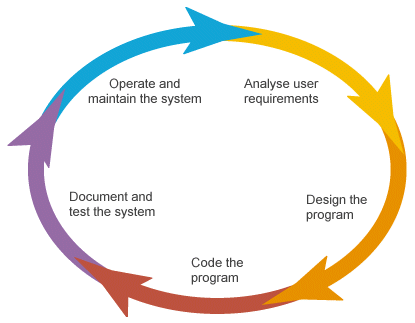
\includegraphics[height=5em]{development_life_cycle.png}
\end{columns}
\end{frame}

\begin{frame}[fragile]
  \frametitle{Il faut bien commencer quelque part}

  \center{Cycle de vie d'un projet}
  \linebreak

\begin{columns}[c]
\column{.75\textwidth} 

  Prenons comme exemple un projet relativement simple, une application web
  dont les besoins évoluent avec le succès grandissant.

  \center{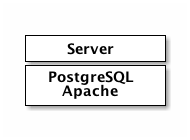
\includegraphics[height=1in]{archi_v1.png}}  

\column{.25\textwidth}
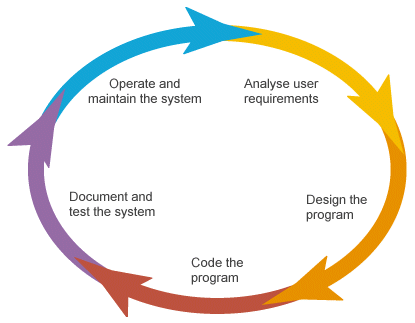
\includegraphics[height=5em]{development_life_cycle.png}
\end{columns}
\end{frame}

\section{Besoins et Architectures}

\subsection{Augmentation du trafic}

\begin{frame}[fragile]
  \frametitle{Séparation des tâches}

  \center{Disponibilité des services}
  \linebreak
  \linebreak

\begin{columns}[c]
\column{.65\textwidth} 

  \begin{itemize}
   \item<1-> partie frontale \textit{stateless}
   \item<2-> attention à \texttt{max\_connections}
   \item<2-> pas de connections persistentes !
   \item<3-> \texttt{pgbouncer}
  \end{itemize}  

\column{.35\textwidth}

\includegraphics[height=4em]{bouncer.png}
\end{columns}
\end{frame}


\frame{
  \frametitle{Séparation des tâches}

  \center{Utilisation de serveurs dédiée et d'un concentrateur de connections}

\begin{center}
  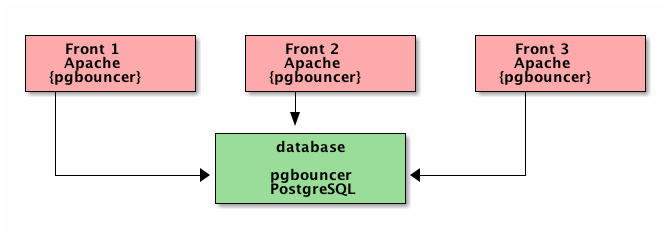
\includegraphics[height=1.3in]{archi_v2.png}
\end{center}  
}

\begin{frame}[fragile]
  \frametitle{pgbouncer}

  \center{\texttt{pgbouncer} réutilise des connexions client \textbf{et} serveur.}

  \only<1>{
    \begin{center}
      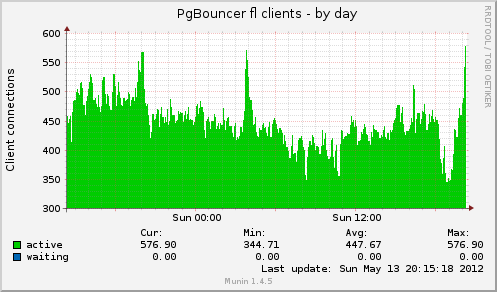
\includegraphics[height=2in]{pgbouncer_db_fl_pools_cl-day.png}
    \end{center}
  }
  \only<2>{
    \begin{center}
      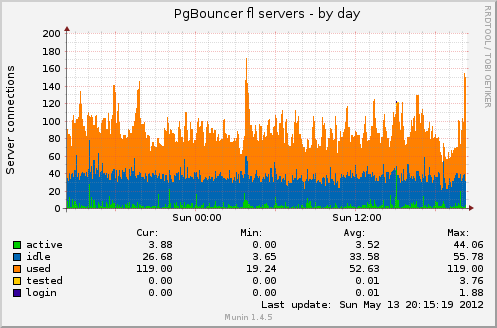
\includegraphics[height=2in]{pgbouncer_db_fl_pools_sv-day.png}
    \end{center}
  }
\end{frame}

\subsection{Durabilité des données}

\begin{frame}[fragile]
  \frametitle{Le plan de sauvegardes}

  \center{Le plan de sauvegardes est crucial}

\begin{columns}[c]
\column{.65\textwidth} 

  \begin{itemize}
   \item<1-> \texttt{pg\_dump -Fc} nocturne
   \item<1-> \texttt{pg\_dumpall --globals-only}
   \item<2-> Rétention des données
   \item<2-> Nocturne, 7 jours
   \item<2-> Hebdomadaire, 7 semaines
   \item<2-> Mensuelle, 12 mois
   \item<3-> Annuelle, 30 ans
  \end{itemize}  

\column{.35\textwidth}
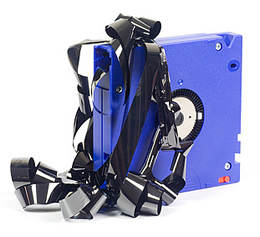
\includegraphics[height=7em]{online-backup.jpg}
\end{columns}
\end{frame}

\begin{frame}[fragile]
  \frametitle{Plan de Reprise de l'Activité}

  \center{\texttt{pg\_dump}, \texttt{pg\_restore}}
  \linebreak
  \linebreak

\begin{columns}[c]
\column{.75\textwidth} 

  \begin{itemize}
    \item<1-> protège contre les \textit{erreurs et omissions}
    \item<1-> temps de restauration conséquent
    \item<2-> Indispensable à la \textbf{durabilité} des données
    \item<2-> ne garanti pas leur \textbf{disponibilité}
  \end{itemize}

\column{.25\textwidth}
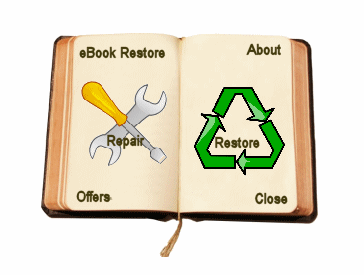
\includegraphics[height=7em]{restore.png}
\end{columns}
\end{frame}

\begin{frame}[fragile]
  \frametitle{Plan de Reprise de l'Activité}

  \center{Sauvegardes physiques et retour à un point dans le passé}

\begin{columns}[c]
\column{.65\textwidth} 

  \begin{itemize}
   \item<1-> \alert{Point In Time Recovery}, 8.1
   \item<2-> \textit{warm standby}, 8.2
   \item<3-> Archivage et \textit{crash recovery}
   \item<3-> \texttt{archive\_command}
   \item<3-> \texttt{restore\_command}
   \item<4-> \texttt{walmgr.py}, {\texttt{WAL-E}
  \end{itemize}  

\column{.35\textwidth}

\includegraphics[height=6em]{pitr.png}
\end{columns}
\end{frame}

\frame{
  \frametitle{Warm Standby}

  \center{Mise en place du Warm Standby}

\begin{center}
  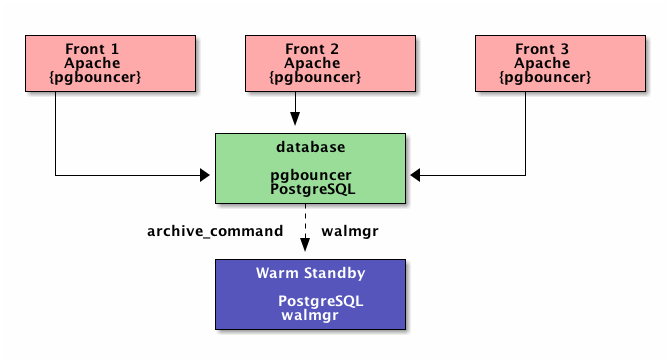
\includegraphics[height=2.1in]{archi_v3.png}
\end{center}    
}

\subsection{Disponibilité des services}

\begin{frame}[fragile]
  \frametitle{Séparation des composants}

  \center{Il est parfois possible de distinguer backoffice et production}
  \linebreak

\begin{columns}[c]
\column{.65\textwidth} 

  \begin{itemize}
   \item<1-> Réplication croisée
   \item<2-> Slony, \textbf{Londiste}, Bucardo
   \item<3-> Traitements spécifiques, \textit{batches}
   \item<3-> Contexte \textit{hors-ligne}
   \item<3-> Traitements \textit{Transactionnels}
   \item<4-> Skytools fourni \alert{\textbf{PGQ}}
  \end{itemize}  

\column{.35\textwidth}

\includegraphics[height=6em]{cross-replication.jpg}
\end{columns}
\end{frame}

\frame{
  \frametitle{Séparation des composants}

  \center{Mise en place de Londiste et PGQ}

\begin{center}
  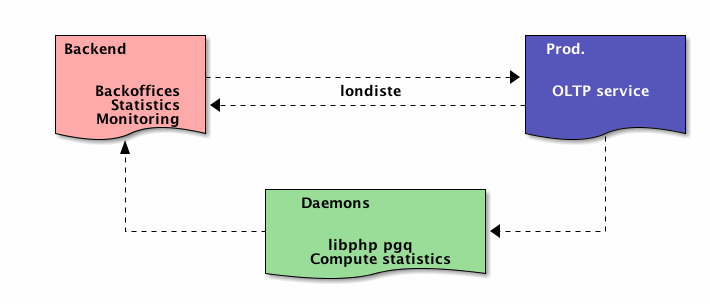
\includegraphics[height=1.7in]{archi_v4.png}
\end{center}    
}

\begin{frame}[fragile]
  \frametitle{Queueing avec PGQ}

  \center{PGQ pour les traitements \textit{hors ligne}}
  \linebreak

\begin{columns}[c]
\column{.6\textwidth} 

  \begin{itemize}
   \item<1-> Écrit principalement en \texttt{PLpgSQL}
   \item<1-> API clientes en \texttt{python}
   \item<1-> et \texttt{PHP}
   \item<2-> en cours de portage vers \texttt{Java}
   \item<3-> Skytools3 : \textbf{Cooperative Worker}
   \item<3-> Fiable, robuste, facile à superviser
  \end{itemize}  

\column{.4\textwidth}

\includegraphics[height=9em]{drop-queue.png}
\end{columns}
\end{frame}

\begin{frame}[fragile]
  \frametitle{Plan de Continuité de l'Activité}

  \center{PostgreSQL 9.1 propose la \textit{Réplication Synchrone} et \textit{Hot Standby}}
  \linebreak

\begin{columns}[c]
\column{.6\textwidth} 

  \begin{itemize}
   \item<1-> \alert{Hot Standby}
   \item<2-> Réplication \textit{(A)}Synchrone
   \item<2-> Connection \texttt{libpq}
   \item<3-> \texttt{recovery.conf}
   \item<3-> Archivage toujours nécessaire
   \item<3-> Activable \textbf{par transaction}
   \item<4-> Bonnes Performances
  \end{itemize}  

\column{.4\textwidth}

\includegraphics[height=9em]{bits.jpeg}
\end{columns}
\end{frame}

\frame{
  \frametitle{Plan de Continuité de l'Activité}
  \center{Mise en place de Hot Standby}
  
\begin{center}
  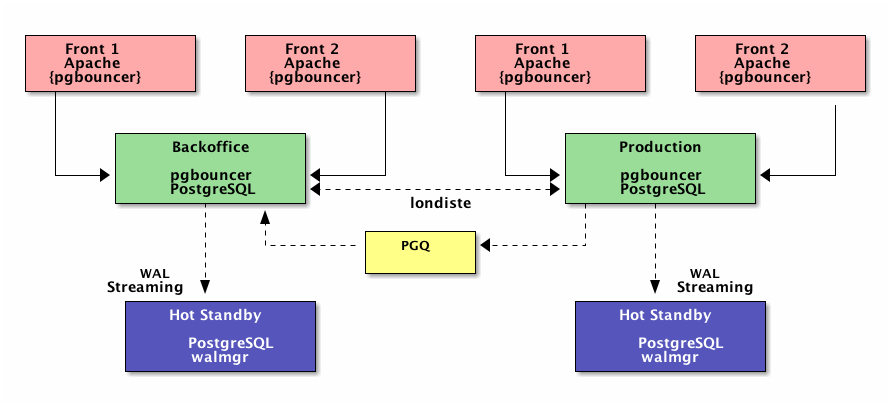
\includegraphics[height=1.9in]{archi_v5.png}
\end{center}
}

\subsection{Sharding}

\begin{frame}[fragile]
  \frametitle{Augmenter la capacité en écriture}

  \center{\texttt{PL/proxy}}
  \linebreak
  \linebreak

\begin{columns}[c]
\column{.6\textwidth} 

  \begin{itemize}
   \item<1-> \textit{Scale-up} ou \textit{Scale-out} ?
   \item<2-> \textit{Remote Procedure Call}
   \item<3-> \textit{Sharding}
   \item<3-> Base de données répartie
   \item<4-> Transactions autonomes
   \item<5-> \textbf{Procédures Stockées}
  \end{itemize}  

\column{.4\textwidth}

\includegraphics[height=9em]{distribution.jpg}
\end{columns}
\end{frame}


\frame{
  \frametitle{Augmenter la capacité en écriture}
  \center{Mise en place de \texttt{plproxy}}

  \only<1>{
    \begin{center}
      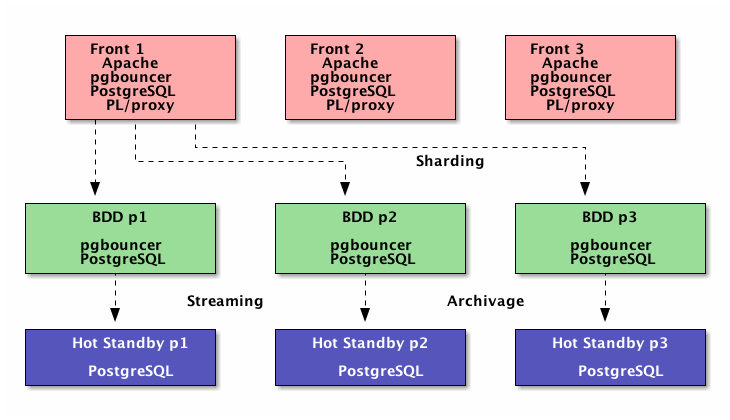
\includegraphics[height=1.9in]{archi_v6.png}
    \end{center}
  }
  \only<2>{
    \begin{center}
      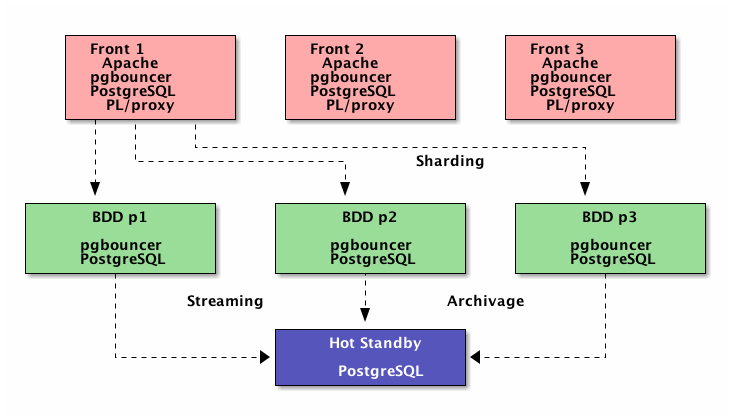
\includegraphics[height=1.9in]{archi_v7.png}
    \end{center}
  }
}

\section{Conclusion}

\subsection{Rétrospective et avenir de la réplication PostgreSQL}

\begin{frame}[fragile]
  \frametitle{Haute Disponibilité Multi Sites}

  \center{Rétrospective et avenir de la réplication dans PostgreSQL}
  \linebreak

\begin{columns}[c]
\column{.55\textwidth} 

  \begin{itemize}
   \item<1-> \textbf{8.1}, PITR
   \item<2-> \textbf{8.2}, Warm Standby
   \item<3-> \textbf{8.3}, \texttt{pg\_standby}
   \item<4-> \textbf{9.0}, Hot Standby
   \item<5-> \textbf{9.1}, Replication Synchrone
   \item<6-> \textbf{9.2}, Replication en Cascade
   \item<7-> \textbf{9.3}, \alert{Bi-Directional Replication}
  \end{itemize}  

\column{.45\textwidth}

\includegraphics[height=9em]{bdr.png}
\end{columns}
\end{frame}

\subsection{Questions}

\frame{
  \frametitle{Questions ?}

\begin{center}
  Retrouvez-nous sur le stand et dans les couloirs !
  \linebreak
  \linebreak

  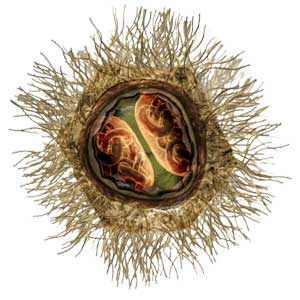
\includegraphics[height=9em]{in-core-replication.jpg}
\end{center}
}

\end{document}
